\setlength{\parskip}{6pt} %% ESPAÇO DEPOIS DE 6pt
\pagenumbering{arabic}  %% PAGINAÇÃO INICIA AQUI

\section{Introdução} \label{sec:int}

Este capítulo apresenta uma pequena introdução que vai ser abordado no decorrer da dissertação, usando modelos de machine learning (aprendizado de máquina), dentro desses modelos vamos abordar a previsão futura dos dados coletados na SANEPAR de Curitiba - PR, esses dados foi coletado no bairro alto, nos anos de 2018 até 2020 houve uma falta de água que afetou todos em Curitiba, afetando não só o bairro alto, mas todos os bairros com o rodízio, de tempos em tempos cada local da cidade tinha água, e outros estavam sem água por um período.

\citeonline{pratica} A previsão tem fascinado as pessoas por milhares de anos, às vezes sendo considerada um sinal de inspiração divina e, às vezes, sendo vista como uma atividade criminosa. O profeta judeu Isaías escreveu em cerca de 700 a.C.

\textit{Diga-nos o que o futuro nos reserva, para que possamos saber que vocês são deuses.
(Isaías 41:23)}

Cem anos mais tarde, na antiga Babilônia, os meteorologistas previam o futuro com base na distribuição de larvas no fígado de uma ovelha podre. Na mesma época, as pessoas que queriam previsões viajavam para Delfos, na Grécia, para consultar o Oráculo, que forneceria suas previsões enquanto intoxicado por vapores de etileno. Os meteorologistas tiveram um momento mais difícil sob o imperador Constâncio, que emitiu um decreto em 357 d.C. proibindo qualquer um ``de consultar um adivinho, um matemático ou um previsor"$\ldots$ 
``Que a curiosidade de prever o futuro seja silenciada para sempre". Uma proibição semelhante de previsão ocorreu na Inglaterra em 1736, quando se tornou uma ofensa fraudar cobrando dinheiro por previsões. A punição foi de três meses de prisão com trabalhos forçados!

As diferentes sortes dos meteorologistas surgem porque as boas previsões podem parecer quase mágicas, enquanto as previsões ruins podem ser perigosas. Considere as seguintes previsões famosas sobre computação.

\begin{itemize}
	\item Há um mercado mundial para talvez cinco computadores. (Presidente da IBM, 1943)
\item Os computadores no futuro não podem pesar mais de 1,5 toneladas. (Mecânica Popular, 1949)
\item Não há razão para alguém querer um computador em sua casa. (Presidente, DEC, 1977)
\end{itemize}
O último deles foi feito apenas três anos antes da IBM produzir o primeiro computador pessoal. Não surpreendentemente, você não pode mais comprar um computador DEC. A previsão é obviamente uma atividade difícil, e as empresas que a fazem bem têm uma grande vantagem sobre aquelas cujas previsões falham.




    \subsection{Contexto da pesquisa} \label{subsec:contexto}
 Em séries temporais, o aprendizado de máquina é frequentemente utilizado para processamento de big data, com o conjunto de dados da SANEPAR em Curitiba - PR, na cidade há algum consumo e escassez de água, é necessário avaliar os dados para ter certeza do que está acontecendo, quando há escassez de água, e picos que ocorrem entre horas e dias.
 
 Dentre os modelos preditivos que serão apresentados em uma revisão sistemática, avaliar o melhor modelo que podemos utilizar e validar quando e como ocorre a escassez de água. Estas análises será em \textit{python}.
 
 Explorar o que são séries temporais e aprendizado de máquina, séries temporais são dados armazenados ao longo do tempo que permitem ao observador analisar anomalias nos dados. Em séries temporais, ordenar os dados por ano ou dia é fundamental e, se os dados atribuídos de forma aleatória, os tomadores de decisão podem cometer erros do tipo. 
 Analisar médias pode ser bem perigoso se não excluir pontos fora da curva também conhecidos como \textit{outliers}. Pode gerar dados muito positivos ou negativos que não correspondem a realidade.
   
      
\subsubsection{Motivação da pesquisa} \label{subsubsec:motivacao}
   %Escrever algo motivador 
    
    De acordo com \cite{vasconcelos_2020} Curitiba e região metropolitana enfrentou um rodízio com $36$ horas com água e $36$ horas sem abastecimento. A média geral dos reservatórios da região está em $27,96\%$ da capacidade. Assim em medida a isso essa pesquisa tem como a abordagem da falta de água, essa falta que pode ser vista como uma seca, em média nos anos anteriores de 2020 a chuva tem marcado a quantia de $1.704$ mm. \cite{vasconcelos_2020} Desde 2016, quando registrou 1.704 mm de chuva, Curitiba não atingiu mais a média anual de precipitação, que é de 1.490 mm, com base em dados da estação pluviométrica do Instituto Nacional de Meteorologia (Inmet).  Apesar de abaixo da média, o mínimo registrado desde então ocorreu em 2020, com 1.158 mm.
    
    Em mediano a essa motivação pode ser melhor interpretado os dados que a SANPEAR ofertor para prever e evitar a escasseia de água que foi registada, e a anomalia que foi detectado em 2020, com a volta da chuva os reservatórios teve aumento do nível.
    
    
    \subsection{Descrição do problema} \label{subsec:descricao}

Nessa subseção vai ser abordado as variáveis do conjunto de dados e como vai ser previsto.

\begin{enumerate}[label={$\blacktriangleright$ }]
\item Bombas de sucção (B1, B2 e B3) – valor máximo da frequência 60 Hz

\item[] Variáveis importantes: Vazão, pressão e nível

\item Nível do Reservatório (Câmara 1) LT01 $ (m^3) $ - \textbf{PREVER}

\item Vazão de entrada (FT01) $ (m^3/h) $

\item Vazão de gravidade (FT02) $ (m^3/h) $

\item Vazão de recalque (FT03) $ (m^3/h) $

\item Pressão de Sucção (PT01SU) (mca)

\item Pressão de Recalque (PT02RBAL) (mca)
\end{enumerate}


Na pesquisa vai ser usado a variável LT01 que é o nível do reservatório, esse nível é de grande importância, como visto nas Figuras \ref{fig:dados-todos} e \ref{fig:2020-a-frente} 

\begin{figure}[H]
	\centering
	\caption{Gráfico dos dados completo em frequência de 24h em media}
	\label{fig:dados-todos}
	\includegraphics[width=1\linewidth]{"Introducao/Figuras/dados todos"}
	
	Fonte: Elaboração própria a partir de dados da SANEPAR (2018 a 2020)
\end{figure}

\begin{figure}[H]
	\centering
	\caption{Ampliando o gráfico no ano de 2020}
	\label{fig:2020-a-frente}
	\includegraphics[width=1\linewidth]{"Introducao/Figuras/2020 a frente"}
	
	Fonte: Elaboração própria a partir de dados da SANEPAR (2018 a 2020)
\end{figure}

Os dados coleatos tem o tamanho de 26306 linhas × 9 colunas, para tanta relação que vai ser usado nos modelos da subseção \ref{subsec:metod} para prever e analisar as anomalias, como apresentado nas Figuras \ref{fig:dados-todos} e \ref{fig:2020-a-frente}.





        
    \subsection{Objetivo geral} \label{subsec:objetivos}

%Escrever melhor dando mais efancie no que vou fazer.
 
Objetivo para essa dissertação é encontrar o melhor modelo de series temporais para o problema de falta d'água que houve em Curitiba.
    
    
    \subsubsection{Objetivos específicos e questão de pesquisa} \label{subsubsec:obespec}
    
Para esse trabalho é pretendente-se busca as anomalias que pode ocorrer nos dados, é porque acontece tais anomalias e responder as questões de pesquisa.

\begin{enumerate}[start=1, label={\textbf{Q} \arabic*}]
	\item \label{q1}  A pressão é suficiente para a demanda diária? 
	\item \label{q2} Quanta água deve ter no reservatório para evitar o acionamento das bombas no horário de pico ($18$ as $21$ h)? Quanto maior a frequência de funcionamento da bomba maior a demanda. Valor máximo $ 60 $ Hz. 
	\item \label{q3} Qual a vazão ótima para atender a demanda? Quanta pressão para atender a demanda? 
	\item \label{q4} Ponto de equilíbrio entre demanda e vazão e ter um armazenamento sem necessidade de acionar as bombas no período do custo energético mais caro ($18$ as $21$ horas).
	\item \label{q5} Se a SANEPAR ativar as bombas de sucção das $18$ às $21$ horas ela tem o maior custo energético, isto é, ela paga mais caro pela energia neste período.
	
	 
	\begin{enumerate}[label=\alph*.]
	\item \label{q5:a} Qual o nível que deve estar no reservatório para não ser necessário a SANEPAR ativar as bombas das $18$ as $21$ horas sem faltar água para a população?
	Verificar a média das vazões nos horários críticos (onde tem a maior demanda $18$ às $21$ horas) para as diferentes estações do ano (Outono, Inverno, Primavera, Verão). 
	\item \label{q5:b} Existe tendência, padrão, sazonalidade para os dados destes 3 anos do Bairro Alto?
	\item \label{q5:c}Identificar quais os horários de maior demanda das $18$ às $21$?
	\item \label{q5:d} Quanto tenho que armazenar previamente no reservatório para não acionar as bombas no horário de pico?
	\item \label{q5:e} Se a vazão cresce e a pressão decresce temos uma ANOMALIA na rede (com base no histórico).	
	\end{enumerate}
\end{enumerate}

    
    \subsection{Procedimentos metodológicos} \label{subsec:metod}

Nessa parte vai ser abordado como será conduzido a dissertação, cada etapa que foi realizado no decorrer das analises feita.
   
    \subsubsection{Etapas da pesquisa}\label{subsubsec:etp}
    A pesquisa se deu seguindo as seguintes etapas:
    
    \begin{enumerate}[start=1, label = {\textbf{Etapa} \arabic* } ]
    	\item Análise exploratória dos dados – EDA ( do inglês \textit{Exploratory Data Analysis}) \label{etp:1}
    	\item O que vai ser usado como variáveis previsoras e qual será a variável a ser predita (MISO) \label{etp:2}
    	\item Fazer a decomposição STL (do inglês \textit{Seasonal-Trend Decomposition}) Sazonalidade, Tendência e Resíduo \label{etp:3}
    	\item Divisão do conjunto de dados em treinamento, validação e teste 70\% para treinamento e validação e 30\% para teste, disso tirando dos 70\% e dividindo em 80\% para treinamento e 20\% para validação. Verificar a média e desvio padrão de cada um destes conjuntos de forma que obtenha a divisão mais adequada dos dados. \label{etp:4}
    	\item Estratégia de previsão (recursiva e iterada-método direto) \label{etp:5}
    	\item Horizonte de previsão (1 passo ou n passos a frente) \label{etp:6}
    	\item Modelos de previsão e métricas de desempenho \label{etp:7}
    	%\item Ajustar os hiperparâmetros dos modelos de previsão Hiperparâmetro ajusta a priori (ex: número de neurônios da rede neural), e parâmetro (pesos da rede neural) ajusta durante o processo. \label{etp:8}
    	\item Aplicar os modelos de previsão e fazer comparativo baseado em testes de significância estatística (\textit{Friedman e Nemenjy}) \label{etp:9}
    \end{enumerate}

\begin{figure}[H]
	\centering
	\caption{Mapa das Etapas}
	\label{fig:etapas}
	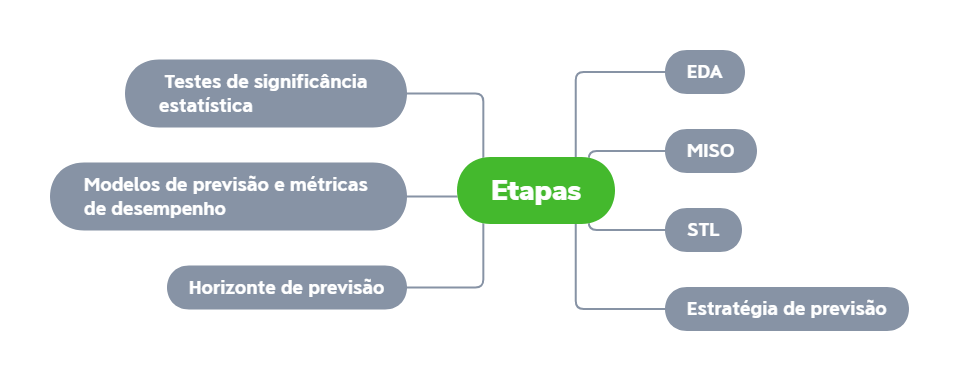
\includegraphics[width=1\linewidth]{Introducao/Figuras/Etapas}
	
	Fonte: Elaboração própria
\end{figure}




    
    
    \subsection{Justificativa da pesquisa} \label{subsec:justif}

No decorrer dessa dissertação ocorre da seguinte forma, para que possa ser previsto e para que seja evitado a efetiva falta d'água, e como pode ser solucionado esse problema para não voltar a acontecer.

\subsubsection{Contribuições} \label{subsubsec:Contribuição}

A água como oxigênio têm uma importância significativa na vida humana, visando isso pode ser notado que sem ela eventualmente não existiria a humanidade, pois segundo \citeonline{walter} A água é a principal substância da vida. O corpo humano é composto de 48 a 54\% de água para pessoas adultas. Com o envelhecimento, a porcentagem de água no corpo humano diminui.

Tendo isso em mente a água que temos hoje pode ser um risco em acabar, como prova \citeonline{vasconcelos_2020} comenta isso no jornal Brasil fato, como os dados dessa pesquisa, vai até o mesmo ano da publicação desse artigo.


    
    \subsection{Estrutura do trabalho} \label{subsec:estrutura}
    Este trabalho está estruturado em~\ref{sec:conclusoes} capítulos, divididos da seguinte forma:
    
    \begin{figure}[H]
    	\centering
    	\caption{Estrutura da dissertação}
    	\label{fig:estrutura}
    	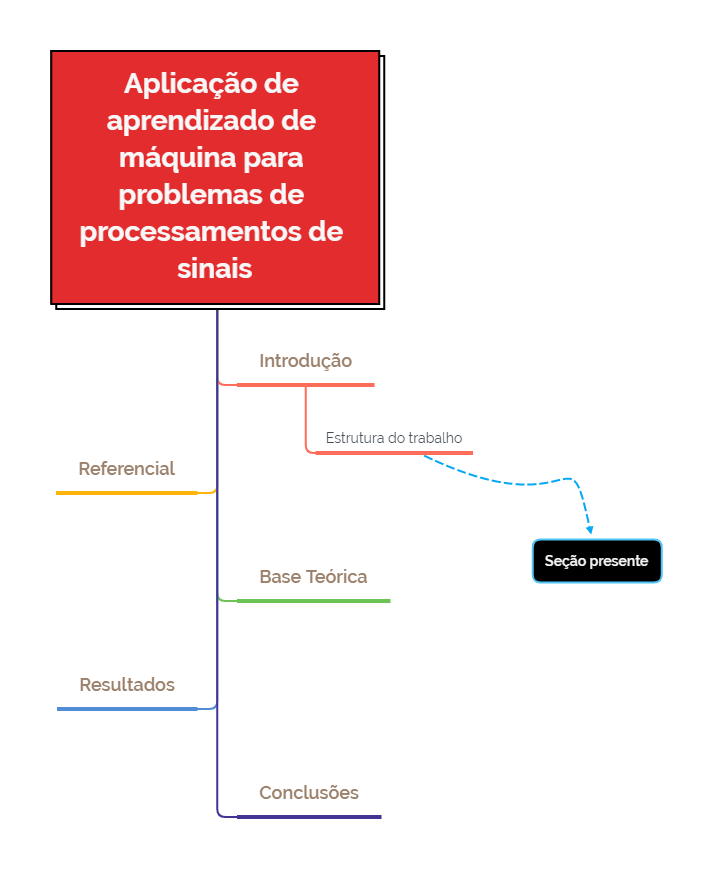
\includegraphics[width=0.7\linewidth]{Introducao/Figuras/Estrutura}
    	
    	Fonte: Elaboração própria 
    \end{figure}
    
    

        O capítulo~\ref{sec:int} apresenta a introdução do trabalho, contendo a contextualização, motivação, objetivo geral, os objetivos específicos, a metodologia utilizada, a justificativa da pesquisa, Contribuições, Publicações e a organização do trabalho.
        O capítulo~\ref{sec:refteo} apresenta a descrição do problema, revisão teórica do trabalho, fazendo um apanhado geral dos principais pesquisadores nos temas abordados na pesquisa.
        O capítulo~\ref{sec:base} apresenta os modelos que será trabalhado nos dados coletado.
        O capítulo~\ref{sec:result} apresenta os resultados da pesquisa, bem como uma análise dos resultados gerado.
        O capítulo~\ref{sec:conclusoes}, por fim, apresenta as considerações finais da pesquisa e algumas propostas de pesquisas futuras.
    
    
    
    